% !TeX TXS-program:compile = txs:///arara
% arara: lualatex: {shell: no, synctex: yes, interaction: batchmode}
% arara: pythontex: {rerun: modified} if exists('pytxcode') && found('pytxcode', 'PYTHONTEX#py')
% arara: lualatex: {shell: no, synctex: yes, interaction: batchmode} if exists('pytxcode') && found('pytxcode', 'PYTHONTEX#py')
% arara: lualatex: {shell: no, synctex: yes, interaction: batchmode} if found('log', '(undefined references|Please rerun|Rerun to get)')

\documentclass[a4paper,11pt]{article}
\usepackage[revgoku]{cp-base}
\graphicspath{{./graphics/}}
%variables
\donnees[
	classe={1\up{ère} 2M2},matiere={[SPÉ.MATHS]},mois=Janvier,annee=2022,typedoc=CHAP,numdoc=5,tailletitre=\LARGE
]
%formatage
\author{Pierquet}
\title{\nomfichier}
\hypersetup{pdfauthor={Pierquet},pdftitle={\nomfichier},allbordercolors=white,pdfborder=0 0 0,pdfstartview=FitH}
\lhead{\entete{\matiere}}
\chead{\entete{\lycee}}
\rhead{\entete{\classe{} - \mois{} \annee}}
\lfoot{\pied{\matiere}}
\cfoot{\logolycee{}}
\rfoot{\pied{\numeropagetot}}
%divers

\begin{document}

\pagestyle{fancy}

\part{CH05 - Probabilités conditionnelles, indépendance - Exercices (Correction)}

\smallskip

\exonum{}

\begin{enumerate}
	\item Compléter le tableau d'effectifs ci-dessous.
	
	\smallskip
	
	\begin{tblr}{%
			width=\linewidth,colspec={l*{4}{X[c]}},
			vline{1}={2-Z}{solid},vline{2-Z}={solid},hline{1}={2-Z}{solid},hline{2-Z}={solid},
			rows={font=\sffamily}
		}
		& Seconde & Première & Terminale & Total\\
		Utilise régulièrement les RS 		&760	&630		&350		&\np{1740} \\
		N'utilise pas régulièrement les RS 	&40		&70			&150		&260 \\
		Total 								&800	&700		&500		&\np{2000} \\
	\end{tblr}
	
	$\blacktriangleright$~~Élèves de terminale : $\dfrac{1}{4} \times \np{2000} = 500$.
	
	$\blacktriangleright$~~Élèves de première : $\dfrac{35}{100} \times \np{2000} = 700$ ; il reste donc  $\np{2000} - (500 + 700) = 800$ élèves en seconde.
	
	$\blacktriangleright$~~Nombre d'élèves de terminale utilisant internet : $\dfrac{70}{100} \times500 = 350$.
	
	$\blacktriangleright$~~Nombre d'élèves de seconde utilisant internet : par différence : $\np{1740} - (350 + 630) = 760$.
	\item La probabilité d'obtenir le questionnaire d'un élève de 2\up{de} qui utilise régulièrement les RS est $\dfrac{760}{\np{2000}} = 0,38$.
	\item On a $P(T) = \dfrac{1}{4} = 0,25$ et  $P_{T}(R) = \dfrac{P(T \cap R)}{P(T)} = \dfrac{\frac{350}{2000}}{\frac{1}{4}} = \dfrac{350}{500} = 0,7$. C'est la probabilité qu'un élève de terminale rencontré au hasard utilise les RS, et cette donnée est dans l'énoncé !
	\item  Sur \np{2000} élèves 260 n'utilisent pas les RS régulièrement. $P\left(\overline{R}\right) = \dfrac{260}{2000} = \dfrac{13}{100} = 0,13$.
	\item Sur les \np{1740} utilisateurs réguliers il y a 630 élèves de première ; la probabilité est donc $P_R(E) = \dfrac{630}{\np{1740}} = \dfrac{21}{58}$.
\end{enumerate}

\medskip

\exonum{}

\begin{enumerate}
	\item On peut proposer l'arbre suivant :
	
	\begin{center}
		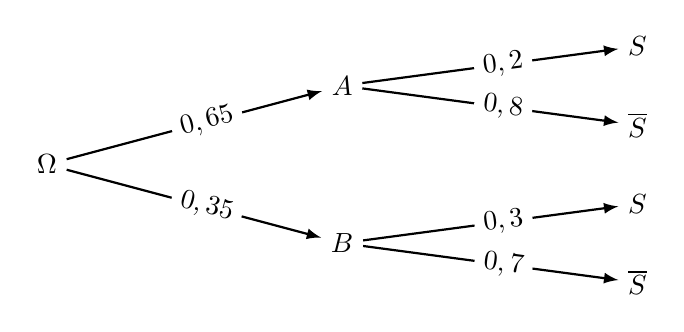
\begin{tikzpicture}[xscale=1,yscale=1]
			\tikzstyle{fleche}=[->,>=latex,thick]
			\tikzstyle{noeud}=[]
			\tikzstyle{feuille}=[]
			\tikzstyle{etiquette}=[pos=0.55,sloped,fill=white]
			
			\def\DistanceInterNiveaux{3}
			\def\DistanceInterFeuilles{1}
			
			\def\NiveauA{(0)*\DistanceInterNiveaux}
			\def\NiveauB{(1.25)*\DistanceInterNiveaux}
			\def\NiveauC{(2.5)*\DistanceInterNiveaux}
			\def\InterFeuilles{(-1)*\DistanceInterFeuilles}
			
			\node[noeud] (R) at ({\NiveauA},{(1.5)*\InterFeuilles}) {$\Omega$};
			\node[noeud] (Ra) at ({\NiveauB},{(0.5)*\InterFeuilles}) {$A$};
			\node[feuille] (Raa) at ({\NiveauC},{(0)*\InterFeuilles}) {$S$};
			\node[feuille] (Rab) at ({\NiveauC},{(1)*\InterFeuilles}) {$\overline{S}$};
			\node[noeud] (Rb) at ({\NiveauB},{(2.5)*\InterFeuilles}) {$B$};
			\node[feuille] (Rba) at ({\NiveauC},{(2)*\InterFeuilles}) {$S$};
			\node[feuille] (Rbb) at ({\NiveauC},{(3)*\InterFeuilles}) {$\overline{S}$};
			
			\draw[fleche] (R)--(Ra) node[etiquette] {${0,65}$};
			\draw[fleche] (Ra)--(Raa) node[etiquette] {${0,2}$};
			\draw[fleche] (Ra)--(Rab) node[etiquette] {${0,8}$};
			\draw[fleche] (R)--(Rb) node[etiquette] {${0,35}$};
			\draw[fleche] (Rb)--(Rba) node[etiquette] {${0,3}$};
			\draw[fleche] (Rb)--(Rbb) node[etiquette] {${0,7}$};
		\end{tikzpicture}
	\end{center}
	\item La probabilité que le questionnaire choisi soit celui d'un employé qui travaille dans le secteur B et qui est stressé est $p(B \cap S)$.
	
	D'après la formule des probabilités composées, $p(B \cap S) = p(B) \times p_{B}(S) = 0,35 \times 0,3 = 0,105$. 
	\item D'après la formule des probabilités totales : $p(S) =  p(A \cap S) + p(B \cap S) = 0,13 + 0,105 = 0,235$.
	
	Le résultat obtenu correspond à 23,5\,\% : la salle de relaxation ne sera pas installée.
	\item Il faut trouver $p_{S}(A) = \dfrac{p(S \cap A)}{p(A)} = \dfrac{0,13}{0,235} \approx 0,55$ au centième près.
\end{enumerate} 

\pagebreak

\exonum{}

\begin{enumerate}
	\item L'énoncé nous donne $p(T) = 0,3$ et  $P_{T}(C)  = 0,6$.
	\item L'arbre de probabilités est : 
	
	\begin{center}
		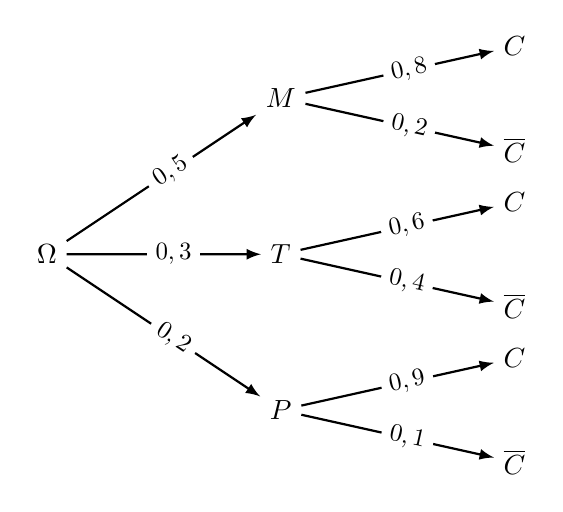
\begin{tikzpicture}[scale=0.66]
			\tikzstyle{fleche}=[->,>=latex,thick]
			\tikzstyle{noeud}=[]
			\tikzstyle{feuille}=[]
			\tikzstyle{etiquette}=[pos=0.55,sloped,fill=white,scale=0.9]
			\tikzstyle{vide}=[]
			\def\DistanceInterNiveaux{3}
			\def\DistanceInterFeuilles{1}
			\def\NiveauA{(0)*\DistanceInterNiveaux}
			\def\NiveauB{(1.5)*\DistanceInterNiveaux}
			\def\NiveauC{(3)*\DistanceInterNiveaux}
			\def\InterFeuilles{(-1)*\DistanceInterFeuilles}
			\node[noeud] (R) at ({\NiveauA},{(4)*\InterFeuilles}) {$\Omega$};
			\node[noeud] (Ra) at ({\NiveauB},{(1)*\InterFeuilles}) {$M$};
			\node[feuille] (Raa) at ({\NiveauC},{(0)*\InterFeuilles}) {$C$};
			\node[feuille] (Rac) at ({\NiveauC},{(2)*\InterFeuilles}) {$\overline{C}$};
			\node[noeud] (Rb) at ({\NiveauB},{(4)*\InterFeuilles}) {$T$};
			\node[feuille] (Rba) at ({\NiveauC},{(3)*\InterFeuilles}) {$C$};
			\node[feuille] (Rbc) at ({\NiveauC},{(5)*\InterFeuilles}) {$\overline{C}$};
			\node[noeud] (Rc) at ({\NiveauB},{(7)*\InterFeuilles}) {$P$};
			\node[feuille] (Rca) at ({\NiveauC},{(6)*\InterFeuilles}) {$C$};
			\node[feuille] (Rcc) at ({\NiveauC},{(8)*\InterFeuilles}) {$\overline{C}$};
			\draw[fleche] (R)--(Ra) node[etiquette] {$0,5$};
			\draw[fleche] (Ra)--(Raa) node[etiquette] {$0,8$};
			\draw[fleche] (Ra)--(Rac) node[etiquette] {$0,2$};
			\draw[fleche] (R)--(Rb) node[etiquette] {$0,3$};
			\draw[fleche] (Rb)--(Rba) node[etiquette] {$0,6$};
			\draw[fleche] (Rb)--(Rbc) node[etiquette] {$0,4$};
			\draw[fleche] (R)--(Rc) node[etiquette] {$0,2$};
			\draw[fleche] (Rc)--(Rca) node[etiquette] {$0,9$};
			\draw[fleche] (Rc)--(Rcc) node[etiquette] {$0,1$};
		\end{tikzpicture}
	\end{center}
	\item 
	\begin{enumerate}
		\item $M \cap C$ représente l'évènement \og le client a pris un macaron \textbf{et} un café \fg.
		
		Et on a $p(M \cap C) = p(M) \times p_M(C) = 0,5 \times 0,8 = 0,4$. 
		\item D'après la formule des probabilités totales, on a $p(C) = p(M \cap C) + p(T \cap C) + p(P \cap C)$.
		
		Et donc $p(C) = 0,4 + 0,3 \times 0,6 + 0,2 \times 0,9 =  0,4 + 0,18 + 0,18 = 0,76$.
	\end{enumerate} 
	\item Il faut trouver $p_C (M) = \dfrac{p(C \cap M)}{p(C)} = \dfrac{0,4}{0,76} \approx 0,53$ à 0,01 près.
	\item
	\begin{enumerate}
		\item On a :
		
		\tabula{}$\bullet~~P + M + C$ : 18 + 6 + 2 = 26~\euro ;
		
		\tabula{}$\bullet~~P + M$ : 18 + 6 = 24~\euro ;
		
		\tabula{}$\bullet~~P + T + C$ : 18 + 7 + 2 = 27~\euro ;
		
		\tabula{}$\bullet~~P + T$ : 18 + 7 = 25~\euro ;
		
		\tabula{}$\bullet~~P + C$  : 18 + 2 = 20~\euro ;
		
		\tabula{}$\bullet~~P$ : 18~\euro
		\item le tableau complété est :
		
		\smallskip
		
		\begin{tabularx}{\linewidth}{|l|*{6}{>{\centering \arraybackslash}X|}}\hline
			Sommes $s_{i}$& 18 &20 &24 &\ldots&\ldots&\ldots\\ \hline
			$p\left(s_{i}\right)$&$0,02$&$0,18$	&$0,1$	&$0,12$	&$0,4$	&$0,18$\\ \hline 
		\end{tabularx}
		
		\smallskip
		\item On a $18 \times 0,02 + 20 \times0,18 + 24 \times0,1 + 25 \times0,12 + 26 \times 0,4 + 27 \times 0,18 = 24,62$~(\euro).
		
		Sur un grand nombre de repas la recette par client s'élève à 24,62~\euro. 
	\end{enumerate}
\end{enumerate}

\end{document}